% !TEX root = ../main.tex

\chapter{Appendix}

\begin{figure}[h!]
  \centering
  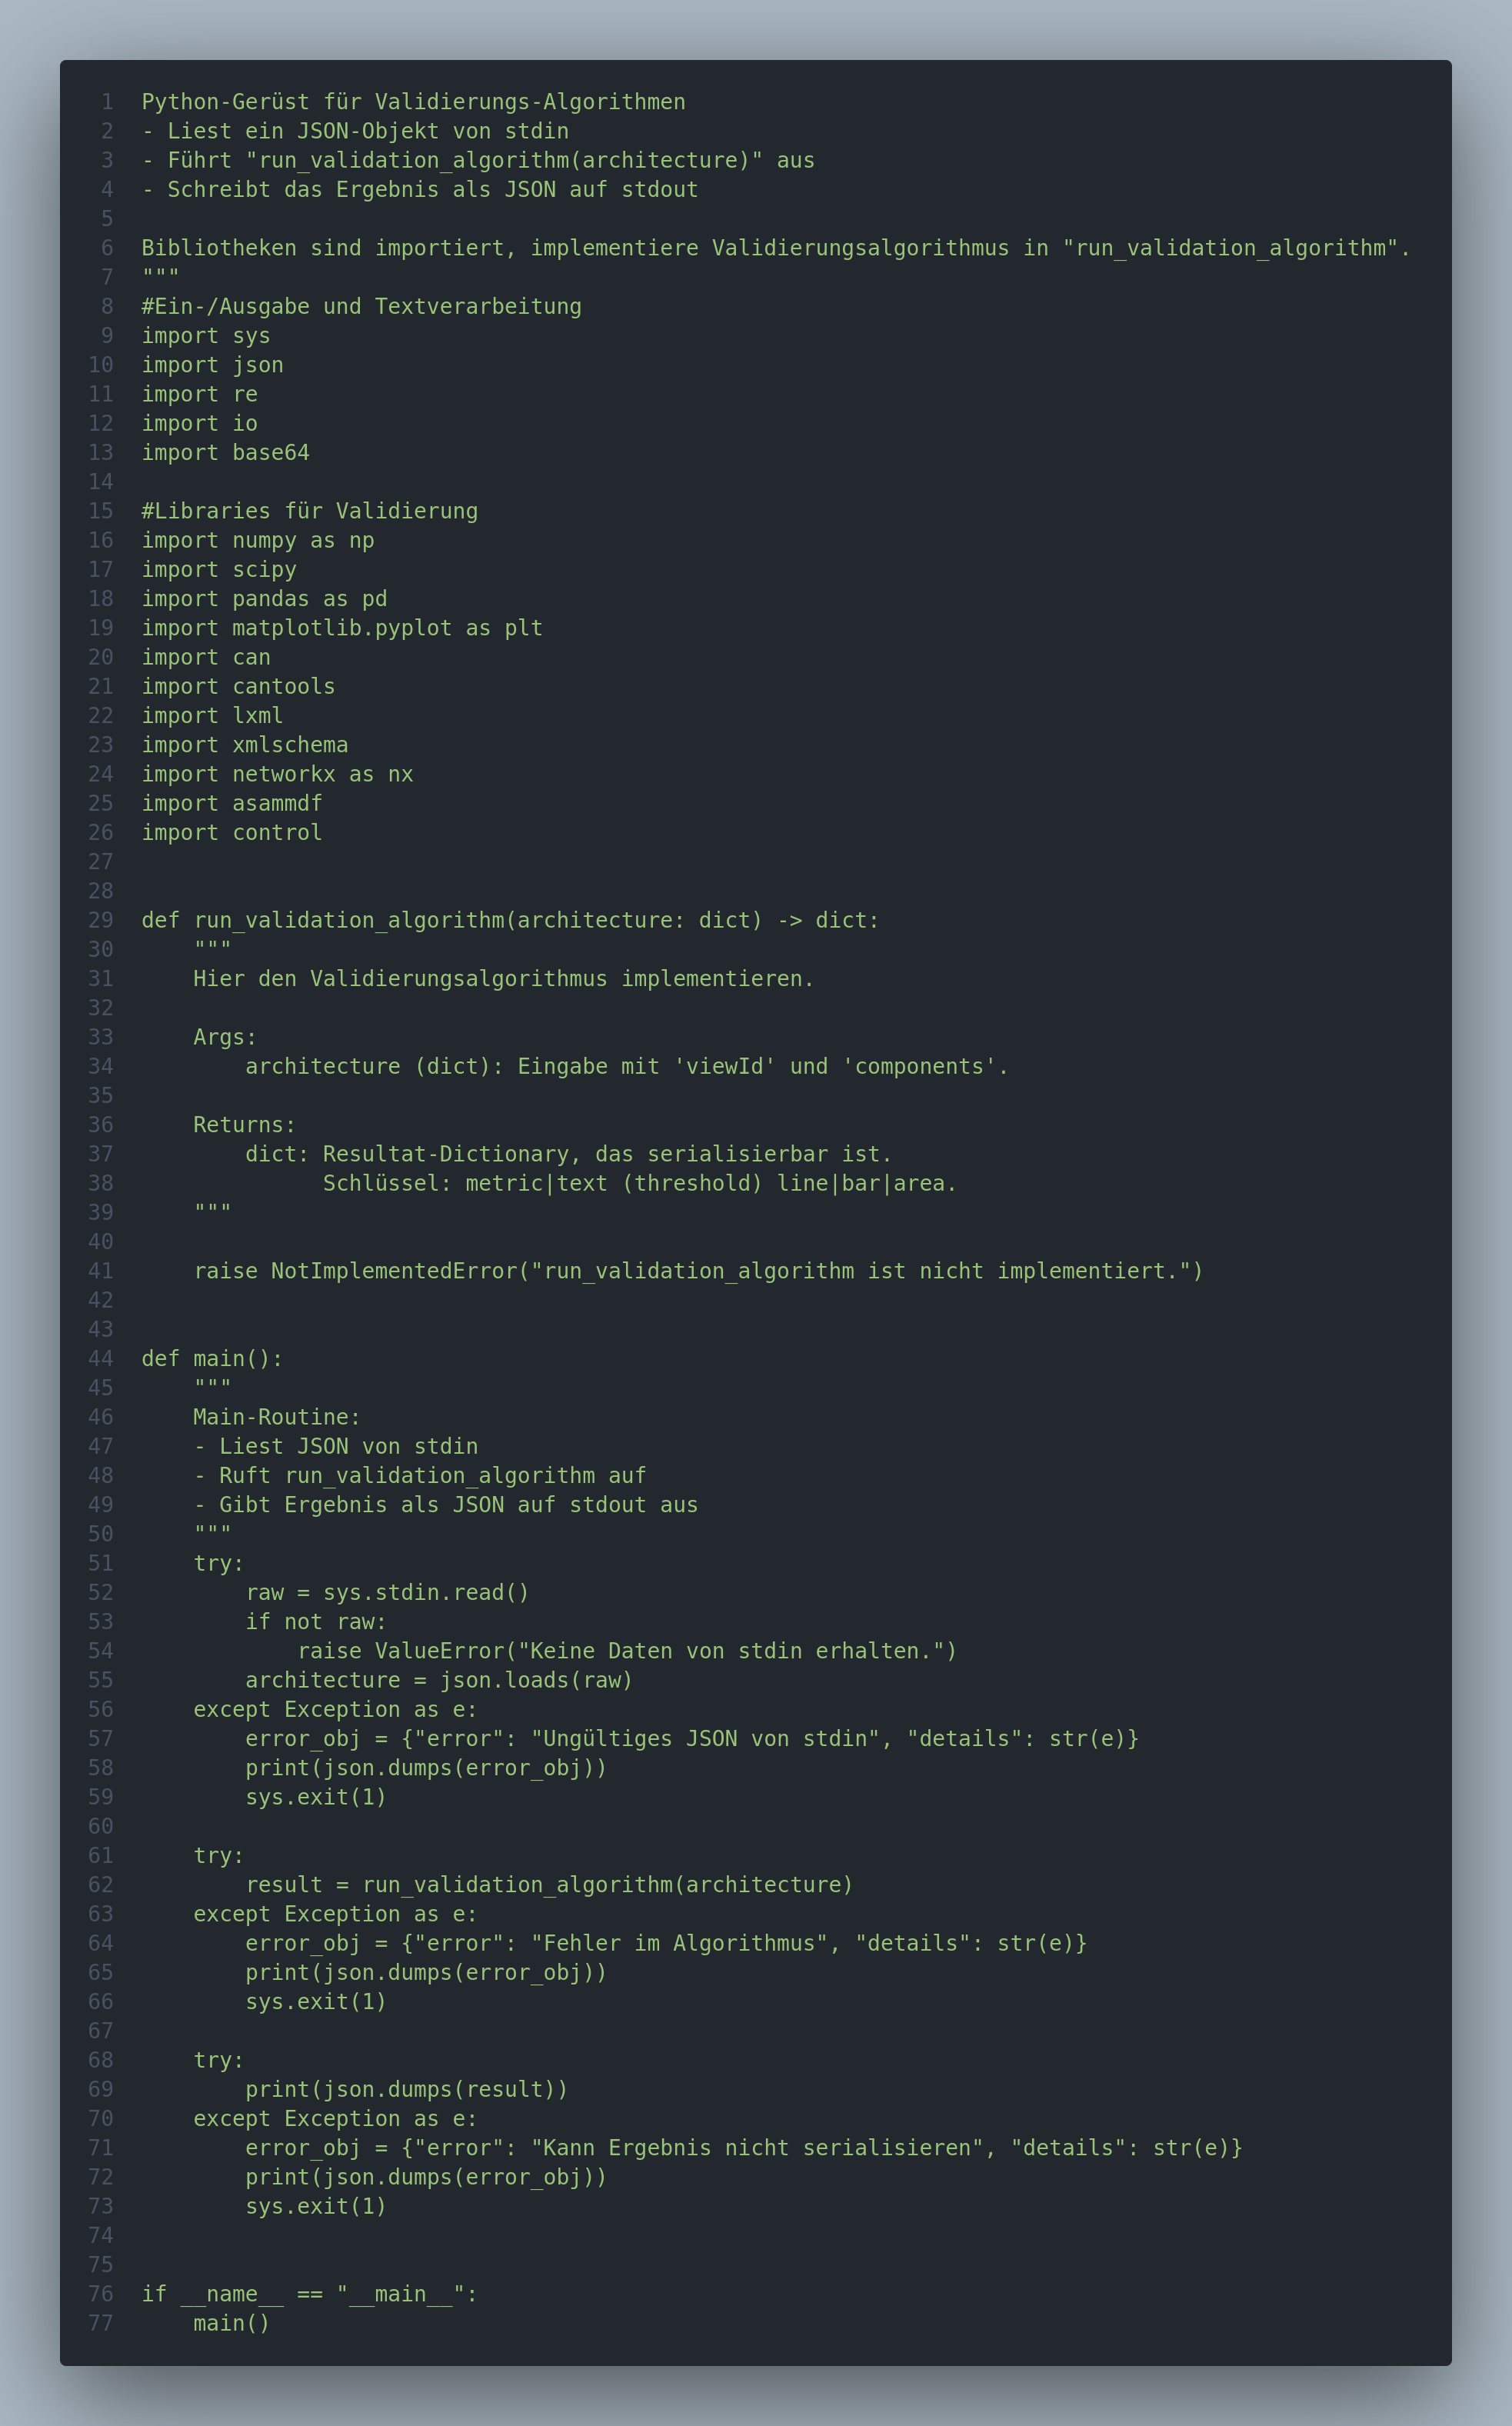
\includegraphics[height=.765\textheight]{figures/05Implementierung/code.png}
  \caption{Python-Codegerüst für die Validierungsalgorithmen}
  \label{fig:codeskeleton}
\end{figure}

\begin{figure}[h!]
  \centering
  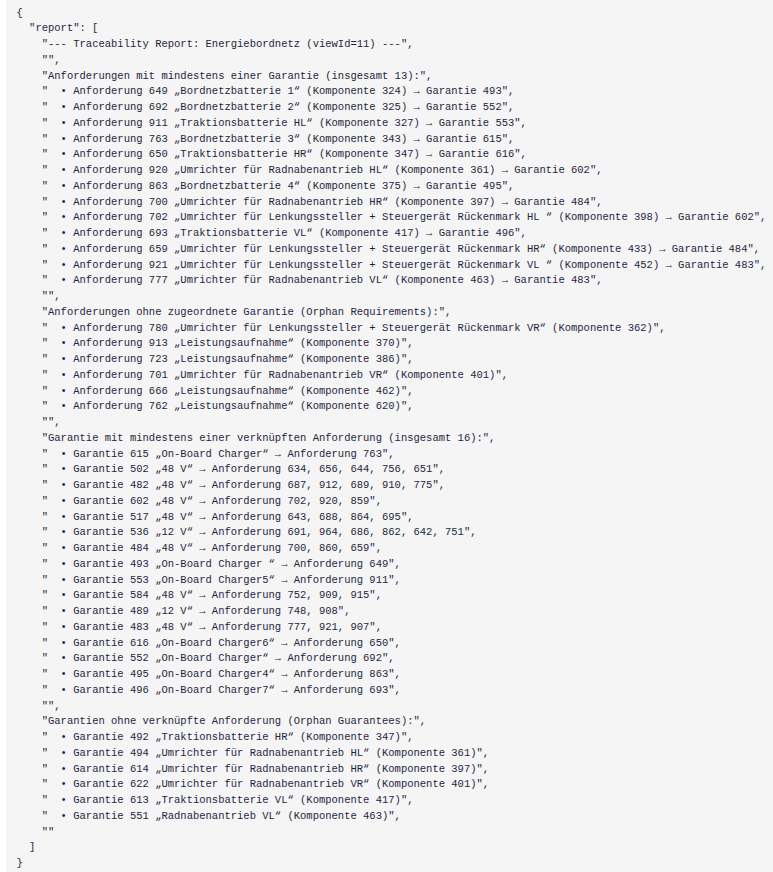
\includegraphics[width=\textwidth]{figures/06Evaluation/Bildschirmfoto vom 2025-06-29 13-23-12.png}
  \caption{Vollständiger Bericht des Traceability-Checks}
  \label{fig:fullresult}
\end{figure}

\begin{figure}[h!]
  \centering
\includegraphics[width=\textwidth]{figures/Appendix/Balken_Fläche.drawio.png}
\caption{Weitere Visualisierungsmöglichkeiten wie Balken-, und Flächendiagramm}
\label{fig:metricvis}
\end{figure}